%% ma: L12-B01-0026
%% lop: 12
%% chuong: 1
%% bai: 1
%% dang: 12.1.3
%% loai: TN4
%% muc: TH
%% dap_an: "C"
%% nguon: "(NBV)-ĐỀ SỐ 16-MỖI NGÀY 1 ĐỀ THI 2025.pdf (D16, MỖI NGÀY 1 ĐỀ - Đề số 16), Phần I Câu 1"
%% kien_thuc: "Bài 1 (tính đơn điệu từ bảng biến thiên)"
%% trang_thai: chinh-thuc
%% ghi_chu: "Đáp án gốc C đúng. Bảng biến thiên có gián đoạn tại x = -1 (hàm không xác định tại điểm này) nên B và D sai. Trùng ý tưởng với dạng đã duyệt 12.1.3, nhập chính thức."
\begin{ex}
Cho hàm số $y=f(x)$ có bảng biến thiên như sau:
\begin{center}
\begin{tikzpicture}
  \tkzTabInit[lgt=1.5,espcl=3.1]{$x$/.8,$f'(x)$/.8,$f(x)$/2.4}{$-\infty$,$-1$,$\dfrac13$,$+\infty$}
  \tkzTabLine{,-,d,-,0,+,}
  \tkzTabVar{+/$+\infty$,-D+/$-\infty$/$+\infty$,-/$\dfrac12$,+/$+\infty$}
\end{tikzpicture}
\end{center}
Khẳng định nào sau đây đúng?
\choice{Hàm số đã cho nghịch biến trên $(-1;+\infty)$}{Hàm số đã cho nghịch biến trên $\left(-\infty;\dfrac13\right)$}{\True Hàm số đã cho đồng biến trên $\left(\dfrac13;+\infty\right)$}{Hàm số đã cho đồng biến trên mỗi khoảng $(-\infty;-1)$ và $\left(\dfrac13;+\infty\right)$}
\loigiai{Từ bảng biến thiên: $f'(x)<0$ trên $(-\infty;-1)$ và trên $\left(-1;\dfrac13\right)$; $f'(x)>0$ trên $\left(\dfrac13;+\infty\right)$.

Hàm số đồng biến trên $\left(\dfrac13;+\infty\right)$, nghịch biến trên mỗi khoảng $(-\infty;-1)$ và $\left(-1;\dfrac13\right)$. A sai vì hàm số đồng biến trên $\left(\dfrac13;+\infty\right)$; B sai vì hàm số không xác định tại $x=-1$; D sai vì hàm số nghịch biến trên $(-\infty;-1)$. Chọn C.}
\end{ex}
